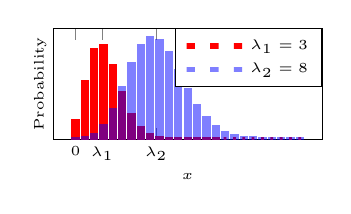
\begin{tikzpicture}
    \tiny
    \begin{axis}[
            xlabel={$x$},
            ylabel={Probability},
            legend style={at={(1,1)},anchor=north east},
            legend style={font=\tiny},
            xtick={0,3,9},
            xticklabels={0,$\lambda_1$,$\lambda_2$},
            ymin  = 0,
            ytick = \empty,
            yticklabel=\empty,
            height = 3cm,
            width = 5cm,
            grid style=dashed,
            bar width=1pt,
        ]
        \addplot [
            domain=0:25,
            samples=25,
            color=red,
            ybar,
            draw opacity=1,
            line width = 2pt,
        ]
        {exp(-3)*(3^x)/(factorial(x))};
        \addlegendentry{$\lambda_1 = 3$}

        \addplot [
            domain=0:25,
            samples=25,
            color=blue,
            ybar,
            draw opacity=0.5,
            line width = 2pt,
        ]
        {exp(-8)*(8^x)/(factorial(x))};
        \addlegendentry{$\lambda_2 = 8$}
    \end{axis}
\end{tikzpicture}